\chapter{The Routing Family}\label{ch:routing}

\begin{quote}\itshape
Variation 2 of the thesis is not ``a model'' but a controlled comparison:
hold the encoder, experts, likelihood, data and evaluation fixed, and vary
only the mechanism that turns gate logits into mixture weights. This
chapter derives each mechanism in the family --- soft, uniform, hard,
top-$k$, Gumbel --- as a small theorem about gradients, including the one
genuine trap (renormalized top-1 looks soft and is provably dead), and
ends with the auxiliary losses and the scope argument that decides where
load balancing is measured. The design payoff is stated up front: because
every mechanism is a pluggable ``prior'' behind one interface, the entire
comparison grid is a config sweep, not a rewrite.
\end{quote}

\section{One interface, five mechanisms}\label{sec:routing-family}

Chapter~\ref{ch:moe} fixed the fused objective
$\NLL = -\LSE_k(\log w_k + \log \gauss_k)$ and left one degree of freedom:
which log-weights $\log w$ enter it. Abstract that choice into a
component --- the package calls it a \code{RegimePrior} --- with the
contract:
\begin{center}
\emph{input:} gate logits $\vz$ (and, for Chapter~\ref{ch:hmm}, a carried
state) \quad $\longmapsto$ \quad
\emph{output:} $\log \pi$ (predictive weights), optionally
$\log \tilde w$ (training weights).
\end{center}
Every mechanism below is one implementation of this contract; the shared
likelihood core and the trainer never change. The five memoryless members,
in one table, each row a theorem proved in this chapter:

\begin{center}
\small
\begin{tabular}{@{}lllll@{}}
\toprule
kind & $\log \pi$ (predictive) & train weights & gate gradient & role \\
\midrule
\code{soft} & $\operatorname{log\_softmax}(\vz)$ & same
  & $\pi - r$ & baseline \\
\code{uniform} & $-\log K$ (frozen) & same
  & $0$ by design & routing-value ablation \\
\code{hard} & one-hot at $\argmax \vz$ & $\log\pi$ masked to argmax
  & $\pi - \bm{e}_{\mathrm{sel}}$ & trainable top-1 \\
\code{topk} & softmax over top-$k$ logits & same
  & alive iff $k \ge 2$ & sparse routing \\
\code{gumbel} & $\operatorname{log\_softmax}\!\bigl((\vz + g)/\tau\bigr)$
  & same & stochastic $\pi - r$ & annealed exploration \\
\bottomrule
\end{tabular}
\end{center}

\begin{engineering}[the ablation grid is a config sweep]
\code{PriorConfig(kind="soft"|"uniform"|"hard"|"topk"|"gumbel"|"hmm")}
selects the mechanism through a registry; nothing else in the system
knows which one is active. This is not convenience --- it is experimental
\emph{validity}. The thesis question ``does routing mechanism X beat Y?''
is only well-posed if X and Y differ in the mechanism alone; the moment
each variant is its own script, the comparison silently absorbs
differences in data handling, initialization, or evaluation. One
interface, many mechanisms, byte-identical everything else --- the same
logic that will make Chapter~16's baselines fair.
\end{engineering}

\section{Soft and uniform: the two ends}\label{sec:softuniform}

\code{soft} is Chapter~\ref{ch:moe} verbatim: $\log \pi =
\operatorname{log\_softmax}(\vz)$, gradient $\pi - r$, the baseline
against which everything else is judged.

\code{uniform} freezes $\log \pi \equiv -\log K$. By
Theorem~\ref{thm:pir}'s derivation the gate gradient is identically zero
--- here \emph{by design}: the mechanism is the control arm that answers
``how much of the mixture's value is the \emph{routing}, as opposed to
merely having $K$ experts and a mixture likelihood?'' The experts still
specialize or not on their own: with uniform weights the responsibilities
reduce to $r_k \propto \gauss_k$, likelihood-ratio assignment, and the
model is an EM mixture with fixed equal weights. If \code{soft} cannot
beat \code{uniform}, the encoder-gate pathway earned nothing on that
panel --- an ablation the thesis must be able to lose honestly
(and one recent MoE-for-finance paper found surprisingly close to a tie,
which is exactly why the arm is in the grid).

\section{Hard routing done right: the hard-EM surrogate}
\label{sec:hardem}

The prototype's sin was not \emph{wanting} winner-take-all routing --- at
deployment, running one expert instead of $K$ is a legitimate wish --- but
implementing the winner selection as an untrainable index operation. The
correct construction keeps hard selection \emph{in the objective}, where
it remains differentiable in the quantities that matter.

Define the hard-EM (classification-EM, Viterbi-training) surrogate:
replace the mixture's $\LSE$ with a max,
\begin{equation}\label{eq:hardem}
  \NLL_{\mathrm{hard}} \;=\; -\max_k\, a_k
  \;=\; -\bigl(\log \pi_{k^\ast} + \log \gauss_{k^\ast}\bigr),
  \qquad k^\ast = \argmax_k a_k,
\end{equation}
i.e.\ score the sample under its single best component, prior included.
Since $\max_k a_k \le \LSE_k(a_k) \le \max_k a_k + \log K$
(Exercise~\ref{ex:6-bound}),
\[
  \NLL \;\le\; \NLL_{\mathrm{hard}} \;\le\; \NLL + \log K:
\]
hard-EM minimizes an upper bound on the true NLL, tight up to $\log K$
nats --- the E-step's soft posterior hardened to an indicator.

The gradient is where the design earns its keep. For fixed selection
$k^\ast$ (locally constant in $\vz$ almost everywhere),
\begin{equation}\label{eq:hardgrad}
  \frac{\partial\, \NLL_{\mathrm{hard}}}{\partial z_k}
  = -\frac{\partial \log \pi_{k^\ast}}{\partial z_k}
  = \pi_k - \delta_{k, k^\ast}
  \;=\; \bigl(\pi - \bm{e}_{k^\ast}\bigr)_k .
\end{equation}
Compare with the prototype's zero. The bare argmax \emph{routed} hard and
carried no objective term in $\pi$; the surrogate scores the selected
branch \emph{including its prior probability} $\log \pi_{k^\ast}$, and
that term is differentiable in every logit. The result is cross-entropy
toward the gate's own argmax --- self-training: confident choices are
reinforced, and the experts' likelihoods feed back through which branch
\emph{wins}. (Switch Transformer's trick --- multiply the selected
expert's output by its gate probability --- is the same maneuver in
point-prediction clothing.)

Two honesty clauses, both visible in the package. First, self-training
can lock in an early wrong choice (the rich-get-richer dynamic of
Section~\ref{sec:loadbalance}); \code{hard} from a cold gate is expected
to glue itself to an arbitrary expert, which is a finding about hard
routing, not a bug. Second --- the interface moral of
Section~\ref{sec:interface} --- the surrogate is for \emph{training
only}: \code{log\_train\_weights} carries the masked
$\log\pi$ that makes \eqref{eq:hardem} the loss, while the predictive
\code{log\_prior} is the honest one-hot (the model claims
$y \sim \gauss(\mu_{k^\ast}, \sigma_{k^\ast}^2)$, full stop), and every
held-out NLL is graded on that claim.

\section{Top-$k$: the trap}\label{sec:topk}

Between soft ($k = K$) and hard ($k = 1$) sits sparse routing: keep the
$k$ largest logits, renormalize among them, zero the rest. In log domain:
mask non-top-$k$ logits to $-\infty$ and \code{log\_softmax} the result;
the $-\infty$ entries drop out of the mixture's $\LSE$ naturally and
receive exactly zero responsibility.

The trap is the $k = 1$ case, and it is worth a formal statement because
it \emph{looks} like a soft, differentiable operation while being exactly
defect 1.

\begin{theorem}[Renormalized top-1 is gradient-dead]\label{thm:topk}
Let $S(\vz)$ be the index set of the $k$ largest logits and
$\tilde\pi_j = e^{z_j} / \sum_{l \in S(\vz)} e^{z_l}$ for $j \in S$, zero
otherwise. If $k = 1$, then away from ties $\tilde\pi = \bm{e}_{k^\ast}$
identically in a neighborhood of $\vz$, and hence
$\partial \tilde\pi / \partial \vz = 0$ almost everywhere --- no gradient
reaches the gate through the mixture weights. If $k \ge 2$, the
within-$S$ Jacobian is that of a $k$-way softmax, which is nonzero
wherever the kept logits are finite and distinct.
\end{theorem}

\begin{proof}
For $k = 1$: on the open set where $z_{k^\ast}$ strictly exceeds all
other logits, $S$ is locally constant, and the renormalized weight is
$e^{z_{k^\ast}} / e^{z_{k^\ast}} = 1$ --- a constant function of $\vz$.
Its derivative is zero there; the tie set where $S$ changes has measure
zero and no derivative at all. For $k \ge 2$: with $S$ locally constant,
$\tilde\pi$ restricted to $S$ is $\operatorname{softmax}(z_S)$, whose
Jacobian $\operatorname{diag}(\tilde\pi) - \tilde\pi\tilde\pi^\top$
vanishes only at vertices of the simplex, unreachable for finite
distinct logits. The mixture weights then depend non-trivially on the
kept logits, and Theorem~\ref{thm:pir}'s computation goes through within
$S$.
\end{proof}

The lesson generalizes the autopsy's: defect 1 was easy to see
(\code{argmax} announces itself); \emph{renormalization after selection
reconstructs the same death silently}, because normalizing a single
survivor erases the very number that carried the gradient. The package
does not document this hazard --- it makes it unrepresentable:
\code{TopKRegimePrior} validates $2 \le k \le K$ at construction and its
error message redirects top-1 seekers to \code{hard}, whose surrogate
supplies the gradient renormalization cannot. (The validation exists
because a test asserting ``top-1 trains the gate'' \emph{failed}; the
theorem above was written after the test, which is the correct order of
events in engineering.) At the other end, $k = K$ keeps every logit and
reduces to \code{soft} exactly --- a free consistency check the test
suite also pins.

\section{Gumbel-softmax: stochastic routing with a temperature}
\label{sec:gumbel}

The mechanisms so far are deterministic. A stochastic gate --- sample a
regime, rather than blend --- brings exploration (early training visits
minority experts) at the price of gradient variance. The classical route
to differentiable sampling is a two-step derivation.

\begin{lemma}[Gumbel-max trick]\label{lem:gumbelmax}
Let $g_1, \dots, g_K$ be i.i.d.\ standard Gumbel
($\Prob(g \le t) = e^{-e^{-t}}$, generated as $-\log(-\log U)$ for
uniform $U$). Then
\[
  \Prob\Bigl(\argmax_k\, (z_k + g_k) = j\Bigr)
  \;=\; \frac{e^{z_j}}{\sum_l e^{z_l}}
  \;=\; \operatorname{softmax}(\vz)_j .
\]
\end{lemma}

\begin{proof}
$j$ wins iff $z_j + g_j > z_l + g_l$ for all $l \ne j$. Condition on
$g_j = t$: the events $\{g_l < z_j - z_l + t\}$ are independent with
probabilities $\exp(-e^{-(z_j - z_l + t)})$. Integrate over the Gumbel
density $e^{-t} e^{-e^{-t}}$:
\[
  \Prob(j \text{ wins})
  = \int_{-\infty}^{\infty} e^{-t} e^{-e^{-t}}
    \prod_{l \ne j} e^{-e^{-(z_j - z_l + t)}}\, dt
  = \int_{-\infty}^{\infty} e^{-t}
    \exp\Bigl(-e^{-t} \underbrace{\textstyle\sum_l
    e^{-(z_j - z_l)}}_{=\,c_j}\Bigr) dt ,
\]
where the sum now includes $l = j$ (its term is $1$). Substitute
$u = e^{-t}$, $du = -e^{-t}dt$: the integral is
$\int_0^\infty e^{-c_j u}\, du = 1/c_j = e^{z_j}/\sum_l e^{z_l}$.
\end{proof}

Sampling a category is thus an argmax over perturbed logits --- which is
again an untrainable index. The relaxation (Jang--Gu--Poole and
Maddison--Mnih--Teh, independently, 2016) replaces that argmax with a
temperature softmax:
\begin{equation}\label{eq:gumbelsoftmax}
  \pi^{(\tau)} \;=\;
  \operatorname{softmax}\!\left(\frac{\vz + \bm{g}}{\tau}\right),
\end{equation}
a \emph{random point on the simplex} that concentrates at a random
vertex as $\tau \to 0$ (recovering exact categorical sampling by the
lemma) and flattens toward uniform as $\tau \to \infty$
(Figure~\ref{fig:gumbel}). Finite $\tau$ buys differentiability ---
gradients flow through \eqref{eq:gumbelsoftmax} into $\vz$ by the
ordinary softmax Jacobian, with the noise acting as a reparameterization
--- at the price of bias (the relaxed weights are not one-hot) and of
gradient variance that grows as $\tau$ falls
(Exercise~\ref{ex:6-tau}). The standard protocol, and the package's,
manages the trade with an \emph{annealing schedule}: start warm
(exploration, low variance), cool exponentially toward a floor,
\[
  \tau(s) \;=\; \tau_{\mathrm{init}}
  \left(\frac{\tau_{\min}}{\tau_{\mathrm{init}}}\right)^{\min(s / S, 1)},
\]
with $s$ the training step. At evaluation the noise and temperature are
dropped entirely --- deterministic
$\operatorname{log\_softmax}(\vz)$ --- because stochastic routing is a
\emph{training} device, and a desk quoting a prediction does not want it
resampled per query.

\begin{figure}[t]
  \centering
  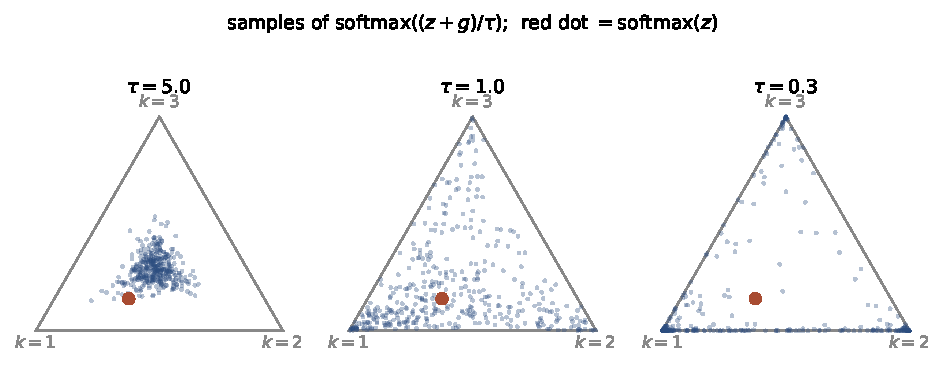
\includegraphics[width=0.92\linewidth]{figures/gumbel_simplex.pdf}
  \caption{\textbf{The temperature knob.} 400 draws of
  $\operatorname{softmax}((\vz + \bm{g})/\tau)$ on the 3-expert simplex,
  fixed logits (red dot $= \operatorname{softmax}(\vz)$). Warm
  ($\tau = 5$): samples hug the mean --- soft routing with jitter. Unit
  temperature: spread across the simplex. Cold ($\tau = 0.3$): mass
  concentrates at the vertices with frequencies approaching
  $\operatorname{softmax}(\vz)$ --- Lemma~\ref{lem:gumbelmax} becoming
  visible. Annealing walks the gate from the left panel to the right one
  over training.}
  \label{fig:gumbel}
\end{figure}

\begin{engineering}[schedules make state, state makes contracts]
The temperature depends on the training step, so the step must reach the
prior: the trainer threads \code{PriorContext(step=step\_count)} into
every forward pass. That one line quietly creates a contract with two
distant subsystems. Determinism: two runs are comparable only if their
schedules align step-for-step --- seeds fix the Gumbel draws, the
threaded step fixes $\tau$. Checkpointing: a resumed run must restore
\code{step\_count} (and the RNG state feeding $\bm{g}$) or the schedule
silently restarts warm and the trajectories diverge --- one of the exact
invariants Chapter~10's bit-identical-resume test pins. A scheduled
quantity is never just a formula; it is state, and state must be owned,
threaded, and persisted.
\end{engineering}

\section{Load balancing, and where to measure it}
\label{sec:loadbalance}

Learned routing has a known instability: \emph{rich-get-richer}. An
expert that wins early gets more gradient, improves faster, and wins
more; its siblings starve at $r_k \approx 0$
(equation~\eqref{eq:mugrad}: no responsibility, no learning). Sparse and
hard variants, which zero out losers entirely, are the most exposed. The
standard counterweight (Shazeer et al.\ 2017) is an auxiliary loss
\begin{equation}\label{eq:lb}
  \mathcal{L}_{\mathrm{lb}}
  \;=\; K \sum_{k} f_k\, \bar p_k,
  \qquad
  \bar p_k = \tfrac{1}{B}\textstyle\sum_b \pi_{bk},
\end{equation}
with $f_k$ the fraction of samples \emph{assigned} to expert $k$
(argmax counts, gradient-stopped) and $\bar p_k$ the mean gate
probability (gradient-carrying). Its gradient pushes probability away
from over-assigned experts; at perfect balance $f_k = 1/K$ the loss is
identically $K \sum_k \bar p_k / K = 1$ \emph{regardless of how sharp
individual rows are} --- balance is enforced marginally, sharpness is
free.

That last property holds only if $f$ is measured over the right pool,
and this is the one place where the finance setting genuinely diverges
from the language-model setting the loss was invented for.

\begin{whatbreaks}[balancing inside a regime-pure batch]
In our panels a batch is often date-sliced, and the regime is a
\emph{date-level} variable: a batch drawn from March 2020 is
legitimately, informatively one-sided. Estimate $f$ on that batch alone
and \eqref{eq:lb} punishes the gate for being right --- it demands
within-date uniformity, which is precisely the sharp regime call the
whole architecture exists to make. Applied naively, the balancing loss
converges the gate toward \code{uniform} and quietly deletes the thesis.
(This is the central warning of arXiv:2501.11873, and our
Chapter~\ref{ch:regimes} persistence math says regime-pure stretches
last \emph{weeks}, so the hazard is the common case, not the corner
case.) The package's \code{LoadBalanceBuffer} therefore accumulates
assignment counts over a rolling window of many batches --- spanning
many dates --- so $f$ estimates the \emph{marginal} utilization across
regimes; a single date remains free to route as one-sidedly as reality
demands. Same formula, different estimator scope, opposite scientific
outcome.
\end{whatbreaks}

Both auxiliary losses in the package (the balance term and an expert
output-decorrelation term aimed at the homogenization failure) default to
\emph{off}: the baseline objective is the pure likelihood, and each aux
term is a pre-registered ablation lever, not silent seasoning. The
buffer, however, always runs --- feeding the utilization dashboard,
because the difference between ``the gate is specializing'' and ``an
expert is dying'' is a monitoring question long before it is a loss
question.

\exercisehead

\begin{exercise}\label{ex:6-bound}
Prove $\max_k a_k \le \LSE(a) \le \max_k a_k + \log K$, and exhibit the
two extreme cases. Conclude the hard-EM objective brackets the true NLL
within $\log K$ nats, and compute what that slack is worth (in NLL units)
for $K = 2$ versus $K = 8$ --- one reason small-$K$ mixtures tolerate
hard training better.
\end{exercise}

\begin{exercise}\label{ex:6-hardgrad}
Derive \eqref{eq:hardgrad} carefully, confirming the likelihood term
contributes nothing to the gate gradient for fixed selection, and show
the expected update direction reinforces the current argmax. Then
describe the fixed points of pure self-training with frozen experts:
which gates are stationary, and why a cold-start gate gluing to an
arbitrary expert is the \emph{generic} outcome rather than bad luck.
\end{exercise}

\begin{exercise}\label{ex:6-topk}
(Hands-on.) Reproduce Theorem~\ref{thm:topk} in six lines of torch:
build $\vz$ with \code{requires\_grad}, mask to top-$k$, renormalize with
\code{log\_softmax}, feed a fused mixture NLL, and print
\code{z.grad} for $k = 1$ and $k = 2$ ($K = 3$). Then explain in one
paragraph why the $k=1$ case cannot be rescued by any smooth
renormalization of a single kept entry --- the information destroyed by
``keep one, normalize'' is not recoverable downstream.
\end{exercise}

\begin{exercise}\label{ex:6-gumbelproof}
Fill in every step of Lemma~\ref{lem:gumbelmax}'s proof: verify the
Gumbel density, the conditioning step, the inclusion of the $l = j$ term,
and the substitution. Then show that $\vz + \bm{g}$ shifted by any
constant leaves the argmax distribution invariant, and connect this to
Exercise~\ref{ex:5-sumzero}'s observation about softmax logits.
\end{exercise}

\begin{exercise}\label{ex:6-tau}
For $K = 2$, write $\pi^{(\tau)}_1 = \operatorname{sigmoid}((\Delta z +
\Delta g)/\tau)$ with $\Delta g$ logistic. (a) Show
$\E[\pi^{(\tau)}] \to \operatorname{softmax}(\vz)_1$ as $\tau \to 0$ and
$\to 1/2$ as $\tau \to \infty$. (b) Simulate the variance of
$\partial \pi^{(\tau)}_1 / \partial \Delta z$ at
$\tau \in \{5, 1, 0.3, 0.1\}$ and describe the trade the annealing
schedule is walking. (c) Why does evaluating with noise on (rather than
the package's deterministic eval mode) make two models' held-out NLLs
incomparable at different $\tau$?
\end{exercise}

\begin{exercise}\label{ex:6-lb}
(a) Verify that \eqref{eq:lb} equals 1 identically under balanced $f$,
for \emph{any} gate matrix --- sharpness is unpenalized. (b) Simulate
rich-get-richer: two experts, one initialized slightly better; train the
mixture NLL without balancing and plot utilization; repeat with
\eqref{eq:lb} under (i) per-batch $f$ on regime-pure batches and (ii)
buffered $f$ spanning both regimes. Confirm (i) destroys sharp routing
while (ii) rescues the starving expert without flattening within-date
decisions --- the package's scope choice, reproduced from scratch.
\end{exercise}
